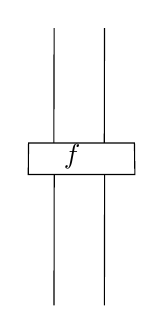
\begin{tikzpicture}[yscale=-1,scale=0.02,baseline={([yshift=-.5ex]current bounding box.center)}]
\begin{scope}[shift={(0.00mm,719.29mm)}]
% path id='path4136'
% path spec='m 527.85715,9.5050806 -2.14286,199.9999994 677.14281,0 L 1200,9.5050756 Z'
\draw [fill=none,draw=black] (527.86mm,9.51mm)
-- ++(-2.14mm,200.00mm)
-- ++(677.14mm,0.00mm)
-- (1200.00mm,9.51mm)
-- cycle
;
% path id='path4140'
% path spec='M 690,-719.06633 688.57143,9.4258293'
\draw [fill=none,draw=black] (690.00mm,-719.07mm)
-- (688.57mm,9.43mm)
;
% path id='path4142'
% path spec='M 1010,-719.06633 1008.5714,9.4258293'
\draw [fill=none,draw=black] (1010.00mm,-719.07mm)
-- (1008.57mm,9.43mm)
;
% path id='path4144'
% path spec='m 690.71579,209.5036 -1.42856,831.5307'
\draw [fill=none,draw=black] (690.72mm,209.50mm)
-- ++(-1.43mm,831.53mm)
;
% path id='path4146'
% path spec='m 1010.7128,209.5036 -1.4286,831.5307'
\draw [fill=none,draw=black] (1010.71mm,209.50mm)
-- ++(-1.43mm,831.53mm)
;
\node [black] at (804.08mm,96.76mm) { $f$ };
\end{scope}
\end{tikzpicture}
